% Include at a fixed width: scaling DOWN would push the
% in-figure type below the 9pt floor the artwork guide sets.
\begin{figure}[t]
  \centering
  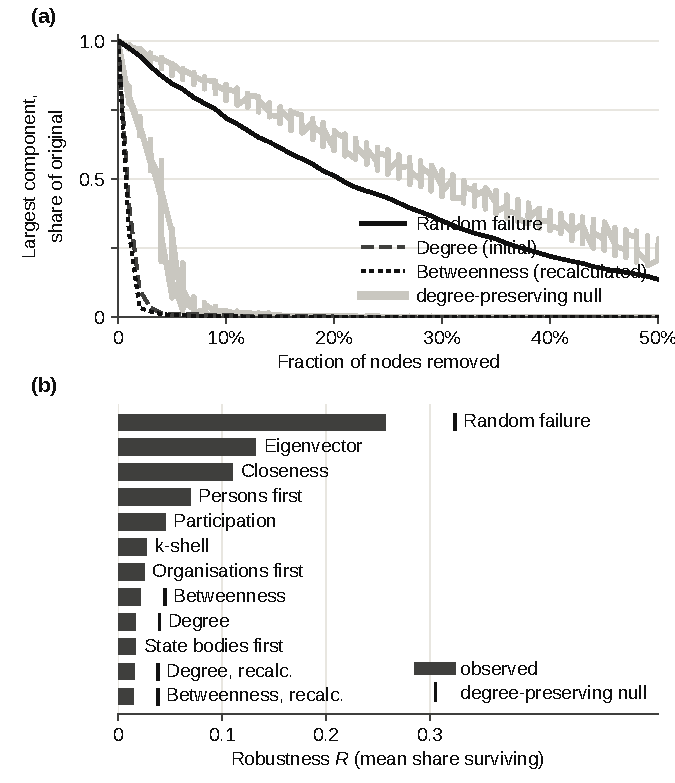
\includegraphics[width=4.5in]{fig17_percolation.pdf}
  \caption{\textbf{The pre-2011 network is as robust to random loss as
  its degree sequence implies, and markedly more vulnerable to targeted
  attack than that sequence requires.}
  Panel (a): the largest connected component as nodes are removed, on the
  2,509-node component of the network evidenced in the \emph{Journal
  Officiel} before 14 January 2011. Shaded bands and their centre lines
  are a degree-preserving configuration-model null over five rewirings;
  random failure is averaged over twenty draws. Panel (b): robustness
  $R$, the mean surviving share over the whole removal sequence
  (Schneider et al. 2011), for every strategy, with the null marked as a
  caliper where it was run.
  Under random failure the observed graph sits on its null
  (0.79$\times$); under targeted attack it falls well below it
  (0.38--0.48$\times$), so the concentration of
  vulnerability is structural and not merely a consequence of the degree
  distribution.
  \textbf{The absolute collapse point should not be read as a finding.}
  This component is very nearly a tree --- 2,921 ties over 2,509 nodes,
  413 independent cycles, 61\% of nodes at degree 1 and 687 articulation
  points --- so it has almost no redundancy to lose and every strategy
  destroys it quickly. What is interpretable is the comparison between
  strategies and against the null. Ownership and kinship ties, the two
  layers most likely to supply the missing redundancy, are absent because
  the roster recording them is undated; this is the resilience of the
  gazette-evidenced network.}
  \label{fig:percolation}
\end{figure}

% ---------------------------------------------------------------------
% Accessibility description (APSR requires one; WCAG 2.1 AA)
% ---------------------------------------------------------------------
% Two greyscale panels. The upper panel plots the surviving share of the
% largest connected component, from 1 down to 0, against the fraction of
% nodes removed, from 0 to 30 per cent. Three observed curves fall: random
% failure declines gradually, while degree-targeted and
% betweenness-targeted removal collapse almost immediately. A pale band
% behind each shows the degree-preserving null; the random curve lies on
% its band and the targeted curves fall below theirs. The lower panel is a
% horizontal bar chart of robustness R for twelve removal strategies,
% ordered from most to least destructive, with a short vertical caliper
% marking the null value on the five bars where a null was computed.
